\scanpage{36}
We shall therefore have additively
\[
(\alpha)\qquad H^*(Y)=\coprod_{\substack{i+j\leq n-1\\i,j\geq0}}L_X^jP^i(X)\oplus E^{n-1}.
\]
The operation
\[\varphi_*:H^*(Y)\longrightarrow H^*(X)\]
is therefore identified with $L_X$ on the piece
\[\coprod_{\substack{i+j\leq n-1\\i,j\geq0}}L_X^jP^j(X)\]
of the first piece of $(\alpha)$, (and is \deleted{\unsure{an isomorphism}} therefore injective on this piece) and it is \uline{zero} on the piece
\[
\deleted{\coprod_{\unsure{0\leq i\leq n-1}}L_X^{\unsure{n-i}}P^i(X)\oplus}E^{n-1},
\]
\deleted{which corresponds \unsure{under the canonical isomorphism} to $\displaystyle\sum_{n-1\leq i\leq2(n-1)}P^i(Y)$}. Thus we find the

\uline{Corollary}
\[
\begin{aligned}
\operatorname{Ker}\varphi_*&=\deleted{\coprod_{\unsure{n-1\leq j\leq2n-1}}P^j(Y)\simeq\operatorname{Ker}}E^{n-1}(Y)\\
\operatorname{Im}\varphi_*&=\operatorname{Im}L_X=\bigcap_{0\leq i\leq n}\operatorname{Ker}p_i^X.
\end{aligned}
\]
(the last formula, since $H^*(Y)=\operatorname{Im}\varphi^*+E^{n-1}$ and $\varphi_*$ vanishes on $E^{n-1}$, hence $\operatorname{Im}\varphi_*=\operatorname{Im}\varphi_*\varphi^*\deleted{=I}$, now $\varphi_*\varphi^*=L_X$).
\[
\left\{\begin{aligned}
p_i^X\varphi_*&=0 &&\text{if }0\leq i\leq n\\
p_{j}^X\varphi_*&=\varphi_*p_{j-2}^Y &&\text{if }n+1\leq i\leq2n.
\end{aligned}\right.
\]
We have
\[
\left\{\begin{aligned}
\varphi^*L_X&=L_Y\varphi^*\\
L_X\varphi_*&=\varphi_*L_Y
\end{aligned}\right.
\qquad
\varphi_*\varphi^*=L_X,\quad\varphi^*\varphi_*=L_Y
\]
projection formula

\margin{\figure{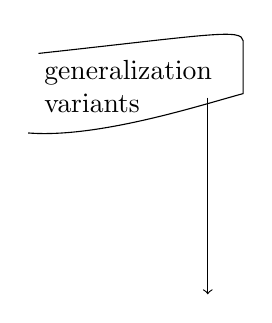
\begin{tikzpicture}[x=1cm,y=1cm]
\node[align=left,anchor=north west] (a) at (0,0) {\deleted{\unsure{generalization}}\\variants};
\draw (-.08,-1.05)..controls(.8,-1.12)and(2.1,-.7)..(2.65,-.55)--(2.65,.12)..controls(2.63,.28)and(2.25,.2)..(.05,-.04);
\draw[->] (2.2,-.6)--(2.2,-3.1);
\end{tikzpicture}}}
\deleted{For the last formula, we note that both sides are zero on $E^{n-1}$, so it suffices to check
\[
(L_X\varphi_*)\varphi^*=(\varphi_*L_Y)\varphi^*\quad\text{i.e.}\quad
L_X(\varphi_*\varphi^*)=\varphi_*(L_Y\varphi^*)=\inserted{\varphi_*\varphi^*L_X}
\]
since both sides are $L_X^2$.}
\mspage{35}
